%%%%%%%%%%%%%%%%%%%%%%%%%%%%%%%%%%%%%%%%%%%%%%%%%%%%%%%%%%%%
%%%%%%%%%%%%%%%%%%%%%%% preamble %%%%%%%%%%%%%%%%%%%%%%%%%%%
%%%%%%%%%%%%%%%%%%%%%%%%%%%%%%%%%%%%%%%%%%%%%%%%%%%%%%%%%%%%

\documentclass[compress,red,12pt]{beamer}
\mode<presentation>
%
% Beamer default paper size is 128mm by 96mm
%

\usetheme{Singapore}
% other themes: AnnArbor, Antibes, Bergen, Berkeley, Berlin,
%               Boadilla, boxes, CambridgeUS, Copenhagen,
%               Darmstadt, default, Dresden, Frankfurt, Goettingen,
%               Hannover, Ilmenau, JuanLesPins, Luebeck, Madrid, Maloe,
%               Marburg, Montpellier, PaloAlto, Pittsburg, Rochester,
%               Singapore, Szeged, classic

\usecolortheme{seahorse}
% color themes: albatross, beaver, beetle, crane, default, dolphin, dov,
%               fly, lily, orchid, rose, seagull, seahorse, sidebartab,
%               structure, whale, wolverine

\usefonttheme{structurebold}
% font themes: default, professionalfonts, serif, structurebold,
%               structureitalicserif, structuresmallcapsserif

%
% uncomment to go automatically to full screen
%
%\hypersetup{pdfpagemode=FullScreen}

% define your own colors:
\definecolor{Red}{rgb}{1,0,0}
\definecolor{Blue}{rgb}{0,0,1}
\definecolor{Green}{rgb}{0,1,0}
\definecolor{magenta}{rgb}{1,0,.6}
\definecolor{lightblue}{rgb}{0,.5,1}
\definecolor{lightpurple}{rgb}{.6,.4,1}
\definecolor{gold}{rgb}{.6,.5,0}
\definecolor{orange}{rgb}{1,0.4,0}
\definecolor{hotpink}{rgb}{1,0,0.5}
\definecolor{newcolor2}{rgb}{.5,.3,.5}
\definecolor{newcolor}{rgb}{0,.3,1}
\definecolor{newcolor3}{rgb}{1,0,.35}
\definecolor{darkgreen1}{rgb}{0, .35, 0}
\definecolor{darkgreen}{rgb}{0, .6, 0}
\definecolor{darkred}{rgb}{.75,0,0}

\xdefinecolor{olive}{cmyk}{0.64,0,0.95,0.4}
\xdefinecolor{purpleish}{cmyk}{0.75,0.75,0,0}

% can also choose different themes for the "inside" and "outside"

% \usepackage{beamerinnertheme_______}
% inner themes include circles, default, inmargin, rectangles, rounded
\useinnertheme{circles}

% \usepackage{beamerouterthemesmoothbars}
% outer themes include default, infolines, miniframes, shadow, sidebar,
%               smoothbars, smoothtree, split, tree
%\useoutertheme{miniframes}

% to have the same footer on all slides
%\setbeamertemplate{footline}[text line]{STUFF HERE!}
%\setbeamertemplate{footline}[text line]{} % makes the footer EMPTY
%\setbeamertemplate{footline}{\scriptsize{\vspace*{0.4cm}\hspace*{0.3cm}\insertframenumber}} 
\setbeamertemplate{footline}{\insertpagenumber}

%
% Automatic Outline
%
\AtBeginSection[section]
{
  \begin{frame}
    \frametitle{Outline}
    \tableofcontents[sectionstyle=show/shaded,subsectionstyle=show/show/hide]
  \end{frame}
}

%
% For speed up of compilation
%
%\includeonlyframes{current}

%%%%%%%%%%%%%%%%%%%%%%%%%%%%%%%%%%%%%%%%%%%%%%%%%%%%%%%%%%%%
%%%%%%%%%%%%%%%%%%%%%%% Pacakges  %%%%%%%%%%%%%%%%%%%%%%%%%%
%%%%%%%%%%%%%%%%%%%%%%%%%%%%%%%%%%%%%%%%%%%%%%%%%%%%%%%%%%%%

%
% include packages
%
\usepackage[latin1]{inputenc}
\usepackage[small]{caption}
\captionsetup{labelformat=empty, labelsep=none}
\usepackage{graphicx}
\graphicspath{{./images/}}
\usepackage{bm}
\usepackage{fancybox}
\usepackage{multimedia}
\usepackage{amsmath}
\usepackage{amssymb}
\usepackage{tikz}
\usetikzlibrary{arrows,shapes}
\tikzstyle{every picture}+=[remember picture]
\tikzstyle{na} = [baseline=-.5ex]
\usepackage{cancel}

\DeclareMathAlphabet\mathbfcal{OMS}{cmsy}{b}{n}

\tikzstyle{nodeblue}=[fill=blue!20, anchor=base, rounded corners=2pt]
\tikzstyle{nodered}=[fill=red!20, anchor=base, rounded corners=2pt]
\tikzstyle{nodegreen}=[fill=green!20, anchor=base, rounded corners=2pt]
\tikzstyle{nodeyellow}=[fill=yellow!20, anchor=base, rounded corners=2pt]

%%%%%%%%%%%%%%%%%%%%%%%%%%%%%%%%%%%%%%%%%%%%%%%%%%%%%%%%%%%%
%%%%%%%%%%%%%%%%%% Custom Commands I Use  %%%%%%%%%%%%%%%%%%
%%%%%%%%%%%%%%%%%%%%%%%%%%%%%%%%%%%%%%%%%%%%%%%%%%%%%%%%%%%%
%
% Note:
% Nice curly font is {\bm{\mathcal{D}}}
%
\newcommand{\Grad}[1]{\bm{\triangledown_{#1}}}
\newcommand{\abbrev}[1]{\rm{#1}}
\newcommand{\argmin}{\mathrm{arg}\min}
\newcommand{\curly}[1]{\left\{#1\right\}}
\newcommand{\roundy}[1]{\left(#1\right)}
\newcommand{\recty}[1]{\left[#1\right]}
\newcommand{\PartDeriv}[2]{\frac{\partial{#1}}{\partial{#2}}}
\newcommand{\vect}[1]{\bm{#1}}
\newcommand{\mat}[1]{\bm{#1}}
\newcommand{\transpose}[1]{{#1}^\intercal}
\newcommand{\derivsym}[1]{\,d{#1}}

%
% Used symbols (only partial for now...)
%
\newcommand{\OpSphere}{\mathbfcal{S}}
\newcommand{\OpRot}{\mathbfcal{R}}
\newcommand{\OpDistance}{\bm{D}}
\newcommand{\OpCumsum}{\mathbfcal{C}}
\newcommand{\OpInt}{\mathbfcal{I}}
\newcommand{\OpCamera}{\vect{\Pi}}
\newcommand{\MaskSun}{\mathbfcal{M}}
\newcommand{\Laplacian}{\mathbfcal{L}}
\newcommand{\OpDiag}[1]{\mathbb{D}\left\{#1\right\}}
\newcommand{\DistSet}{\mathcal{C}}
\newcommand{\DistUnknown}{\vect{n}}
\newcommand{\DistEstimated}{\hat{\vect{n}}}
\newcommand{\CostFunc}[1]{E(#1)}

%%%%%%%%%%%%%%%%%%%%%%%%%%%%%%%%%%%%%%%%%%%%%%%%%%%%%%%%%%%%
%%%%%%%%%%%%%%%%%% title page information %%%%%%%%%%%%%%%%%%
%%%%%%%%%%%%%%%%%%%%%%%%%%%%%%%%%%%%%%%%%%%%%%%%%%%%%%%%%%%%

\title[3D Aerosol Recovery]{
  Lightfield Analysis and Recovery of the Atmosphere
}

\author[Amit Aides]{
  Student: Amit Aides \\
  Supervisor: Prof. Yoav Y. Schechner
}

\date{12 September 2013}

%%%%%%%%%%%%%%%%%%%%%%%%%%%%%%%%%%%%%%%%%%%%%%%%%%%%%%%%%%%%
%%%%%%%%%%%%%%%%%%%%%%% begin %%%%%%%%%%%%%%%%%%%%%%%%%%%%%%
%%%%%%%%%%%%%%%%%%%%%%%%%%%%%%%%%%%%%%%%%%%%%%%%%%%%%%%%%%%%

\begin{document}

\begin{frame}
  \titlepage
\end{frame}

%%%%%%%%%%%%%%%%%%%%%%%%%%%%%%%%%%%%%%%%%%%%%%%%%%%%%%%%%%%%
%%%%%%%%%%%%%%%%%%%%%%%%%%%%%%%%%%%%%%%%%%%%%%%%%%%%%%%%%%%%

\section{Introduction}

\begin{frame}{}
  \begin{center}
    {\huge Introduction}
  \end{center}
\end{frame}

%%%%%%%%%%%%%%%%%%%%%%%%%%%%%%%%%%%%%%%%%%%%%%%%%%%%%%%

\subsection{Motivation}

\begin{frame}{Aerosols in the Atmosphere}
  \setbeamercovered{transparent}
  \begin{overlayarea}{\textwidth}{3cm}
    \begin{itemize}
    \item<1-> Fine solid particles or liquid droplets suspended in the
      atmosphere
    \item<2-> Affects the health of Earth's inhabitants
    \item<3-> Affects Earth's climate
    \end{itemize}
  \end{overlayarea}
  \begin{overlayarea}{\textwidth}{4cm}
    \begin{center}
      \includegraphics<1>[width=\columnwidth]{images/aerosol_micrographs.jpg}
      \includegraphics<2>[height=4cm]{images/shenzen_haze.jpg}
      \includegraphics<3>[height=4cm]{images/radiation_budget.jpg}
    \end{center}    
  \end{overlayarea}
  \begin{flushright}
    \only<1-2> {\tiny images taken from
      http://earthobservatory.nasa.gov/Features/Aerosols/}
    \only<3> {\tiny image taken from
      http://calipsooutreach.hamptonu.edu/index.html}
  \end{flushright}
\end{frame}

%%%

\begin{frame}{Eyjafjallaj\"{o}kull Eruption in 2010}
  \begin{center}
    \includegraphics<1>[height=6cm]{images/1024px-Eyjafjallajokull_volcano_plume.jpg}
    \includegraphics<2>[height=6cm]{images/Volcanic_Lavender.jpg}
    \includegraphics<3>[height=6cm]{images/volcano-airport.jpg}
  \end{center}
  \begin{flushright}
    \only<1> {\tiny image taken from http://www.wikipedia.com/}
    \only<2> {\tiny image taken from http://www.wikipedia.com/}
    \only<3> {\tiny image taken from http://www.metrolic.com/eyjafjallajokull-is-dormant...for-the-moment-2042/}
  \end{flushright}
\end{frame}

%%%%%%%%%%%%%%%%%%%%%%%%%%%%%%%%%%%%%%%%%%%%%%%%%%%%%%%

\subsection{Suggested Method}

\begin{frame}{Multi-angle Tomographic Reconstruction}
  \begin{center}
    \only<1>
    {\includegraphics[height=7cm]{images/camera_network-0.png}}
    \only<2>
    {\includegraphics[height=7cm]{images/camera_network-1.png}}
  \end{center}
\end{frame}

%%%

\begin{frame}{Multi-angle imaging from the ground}
  \begin{columns}[T]
    \begin{column}{.5\textwidth}
      \begin{itemize}
      \item Use standard cameras
      \item Visible spectrum
      \item Based on Sun light scattering and attenuation
      \end{itemize}
    \end{column}
    \begin{column}{.5\textwidth}
      \centering
      {\includegraphics[height=3cm]{images/camera_network-1.png}}
    \end{column}
  \end{columns}
\end{frame}

%%%

\begin{frame}[label=current]{Reconstructed Aerosols}
\end{frame}

%%%

\begin{frame}[label=current]{Reconstructed Clouds}
  \centerline{
    \movie[height=7cm, width=12cm, poster, autostart]{Cloud Reconstruction}{clouds.avi}
  }
\end{frame}

%%%%%%%%%%%%%%%%%%%%%%%%%%%%%%%%%%%%%%%%%%%%%%%%%%%%%%%

\subsection{Current Recovery Methods}

\begin{frame}{Remote Sensing}
  \begin{itemize}
  \item<1> MISR - Multi-angle Imaging SpectroRadiometer
  \end{itemize}

  \begin{center}
    \includegraphics<1>[width=\columnwidth]{images/misr.pdf}
  \end{center}

  \begin{flushright}
    \only<1> {\tiny images taken from http://www-misr.jpl.nasa.gov/}
  \end{flushright}
\end{frame}

%%%

\begin{frame}{LIDAR - Light Detection And Ranging}
  \begin{itemize}
  \item<1> From the ground
  \item<2> From space
  \end{itemize}

  \begin{center}
    \includegraphics<1>[width=\columnwidth]{images/lidar.pdf}
    \includegraphics<2>[height=5cm]{images/calipso.jpg}
  \end{center}

  \begin{flushright}
    \only<1> {\tiny images taken from
      http://jp.hamamatsu.com/en/rd/technology/energy/lidar.html}
  \end{flushright}
\end{frame}

%%%

\begin{frame}{Common Atmospheric Models}
  \begin{itemize}
  \item<1> 1D or 2D models
  \end{itemize}

  \begin{center}
    \includegraphics<1>[height=6cm]{images/atmosphere_layer.jpg}
  \end{center}

  \begin{flushright}
    \only<1> {\tiny image taken from the Stratospheric Ozone Electronic Textbook}
  \end{flushright}
\end{frame}

%%%%%%%%%%%%%%%%%%%%%%%%%%%%%%%%%%%%%%%%%%%%%%%%%%%%%%%

\subsection{Related Work}

\begin{frame}{Integral Imaging}
  \begin{columns}[T]
    \begin{column}{.7\textwidth}
      \begin{itemize}
      \item Sample light in space and direction
      \item Enables re-focus, depth recovery, etc
      \end{itemize}
    \end{column}
    \begin{column}{.3\textwidth}
      \centering
      \includegraphics[height=0.30\textheight]{stanford_camera_array_640x480.jpg}
      \captionof{figure}{\tiny http://graphics.stanford.edu/}
      \includegraphics[height=0.30\textheight]{lytro.jpg}
      \captionof{figure}{\tiny http://graphics.stanford.edu/}
    \end{column}
  \end{columns}
\end{frame}

%%%

\begin{frame}{Computed Tomography}
  \begin{columns}[T]
    \begin{column}{.7\textwidth}
      \begin{itemize}
      \item Reconstruct 3D object from a set of projections
      \item Usually assumes attenuation
      \item Optical Tomography assumes a scattering medium
      \end{itemize}
    \end{column}
    \begin{column}{.3\textwidth}
      \centering
      \includegraphics[height=0.40\textheight]{ct.jpg}
      \captionof{figure}{}
      \includegraphics[height=0.30\textheight]{Optical_Tomography.png}
      \captionof{figure}{}
    \end{column}
  \end{columns}  
\end{frame}

%%%

\begin{frame}[T]{Tomographic Reconstruction of Gas Plumes}
  \begin{columns}[T]
    \begin{column}{.7\textwidth}
      \begin{itemize}
      \item Usually done in UV range
      \item Simpler transfer model:
        \begin{itemize}
        \item Only scattering
        \item Only emission and attenuation
        \end{itemize}
      \end{itemize}
    \end{column}
    \begin{column}{.3\textwidth}
      \includegraphics[height=0.40\textheight]{gas.jpg}
      \captionof{figure}{\tiny Cosofret at el. 2009}
    \end{column}
  \end{columns}    
\end{frame}

%%%%%%%%%%%%%%%%%%%%%%%%%%%%%%%%%%%%%%%%%%%%%%%%%%%%%%%%%%%%
%%%%%%%%%%%%%%%%%%%%%%%%%%%%%%%%%%%%%%%%%%%%%%%%%%%%%%%%%%%%

\section{Theory}

%%%%%%%%%%%%%%%%%%%%%%%%%%%%%%%%%%%%%%%%%%%%%%%%%%%%%%%

\subsection{Radiative Transfer}

\begin{frame}{Radiation}
  Light interaction with the atmosphere:
  \begin{itemize}
  \item Loses energy to absorption
  \item Gains energy by emission
  \item Redistributes energy by scattering
  \end{itemize}
  \begin{align*}
    \hat{\Omega} \cdot \nabla I &+ (k_{s}+k_{a}) I_\nu = \\
    &j + \frac{1}{4\pi} \int_\Omega I \cdot P(\hat{\Omega},\Omega) d\Omega
  \end{align*}    
\end{frame}

%%%

\begin{frame}{Absorption}
  \begin{itemize}
  \item  Light is attenuated according to {\em Beer-Lambert} law
  \end{itemize}
  \centerline{\includegraphics<1>[width=0.6\columnwidth]{images/beer_lambert.pdf}}
  \begin{block}{Optical Depth}    
    Measures transparency of medium
    \begin{align*}
      \tau = \sigma \int_{0}^x N(\tilde{x})\derivsym{\tilde{x}}
    \end{align*}
  \end{block}
\end{frame}

%%%

\begin{frame}[T]{Scattering}
  \begin{columns}[T]
    \column{0.6\columnwidth}
    \setbeamercovered{transparent}
    Scattering depends on:\\
    \begin{itemize}
    \item Particle type
    \item Particle Shape
    \item Particle size to wavelength ratio
    \end{itemize}
    \column{0.4\columnwidth}
    \centering
    \includegraphics[height=0.30\textheight]{images/scattering_spheric.jpg}
    \captionof{figure}{\footnotesize Spherical Aerosol}
    \includegraphics[height=0.30\textheight]{images/scattering_nonspheric.jpg}
    \captionof{figure}{\footnotesize Non-spherical Aerosol}
  \end{columns}
\end{frame}

%%%

\begin{frame}{Phase Function}
    \begin{overprint}
      \only<1>
      {\centerline{\def\svgwidth{0.5\linewidth}\small{\input{images/phase_function1.pdf_tex}}}}
      \only<2>
      {\centerline{\def\svgwidth{0.5\linewidth}\small{\input{images/phase_function2.pdf_tex}}}}
      \only<3>
      {\centerline{\def\svgwidth{0.5\linewidth}\small{\input{images/phase_function3.pdf_tex}}}}
    \end{overprint}  
\end{frame}

%%%

\begin{frame}[T]{Phase Function Used}
  \begin{columns}[T]
    \column{0.7\textwidth}
    \begin{itemize}
    \item Rayleigh - for air molecules
    \item Mie - for aerosols
      \begin{itemize}
      \item Approximated using Henyey-Greenstein equation
      \end{itemize}
    \end{itemize}
    \column{0.3\textwidth}
    \centering
    \includegraphics[height=4cm]{images/Mie_Rayleigh.jpg}
  \end{columns}
\end{frame}

%%%

\begin{frame}{Tomography}
  \begin{center}
    \includegraphics<1>[height=6cm]{images/ct.png}
  \end{center}
  
  \begin{flushright}
    \only<1> {\tiny http://medical-dictionary.thefreedictionary.com}
  \end{flushright}
\end{frame}

%%%%%%%%%%%%%%%%%%%%%%%%%%%%%%%%%%%%%%%%%%%%%%%%%%%%%%%%%%%%
%%%%%%%%%%%%%%%%%%%%%%%%%%%%%%%%%%%%%%%%%%%%%%%%%%%%%%%%%%%%

\section{Current PhD Research: Ongoing}

%%%%%%%%%%%%%%%%%%%%%%%%%%%%%%%%%%%%%%%%%%%%%%%%%%%%%%%

\subsection{Image formation using the single-scattering model}

\begin{frame}{Model}
  \begin{columns}[c]
    \column{0.5\columnwidth}
    \setbeamercovered{transparent}
    \begin{itemize}
    \item <1-2> Atmosphere volume
    \item <1-2> Voxel - Volume Element
    \item <3-4> Light is attenuated due to scattering and absorption
    \item <3-5> Light scatters only once between source and viewer
    \item <6> Simple forward model
    \item <6> No Multi-Scattering
    \end{itemize}

    \column{0.5\columnwidth}
    \begin{overlayarea}{\columnwidth}{8cm}
      \only<1> {\centerline{\includegraphics[width=\columnwidth]
          {images/atmo_settings3D1.pdf}}}
      \only<2> {\centerline{\includegraphics[width=\columnwidth]
          {images/atmo_settings3D2.pdf}}}
      \only<3> {\centerline{\includegraphics[width=\columnwidth]
          {images/atmo_settings3D3.pdf}}}
      \only<4> {\centerline{\includegraphics[width=\columnwidth]
          {images/atmo_settings3D4.pdf}}}
      \only<5> {\centerline{\includegraphics[width=\columnwidth]
          {images/atmo_settings3D5.pdf}}}
      \only<6> {\centerline{\includegraphics[width=\columnwidth]
          {images/atmo_settings3D6.pdf}}}
    \end{overlayarea}
  \end{columns}
\end{frame}

%%%

\begin{frame}{Image Formation Model}
  \begin{columns}[c]

    \column{0.7\textwidth}
    \begin{itemize}
    \item <3-> Attenuation \tikz[na] \node[coordinate] (s2) {};
    \item <4-> Scattering \tikz[na] \node[coordinate] (s3) {};
    \end{itemize}

    % \small
    \footnotesize
    \begin{align*}
      \mathrm{I} &= \\
      & \tikz[baseline]{ \node[nodeblue] (d1) {$\mathrm{L}^{\rm TOA}$}; } \,
      \tikz[baseline]{ \node[nodered] (d4) {$\OpCamera$}; }
      \curly{\roundy{
          \tikz[baseline]{ \node[nodegreen] (d3) {$\vect{\alpha}^{\rm aerosol} + \vect{\alpha}^{\rm air}$}; } }  \odot 
        \tikz[baseline]{ \node[nodeyellow] (d2) {$\exp^{-(\vect{\tau}^{\rm aerosol} + \vect{\tau}^{\rm air})}$}; } }
    \end{align*}
    \normalsize

    \begin{itemize}
    \item <2-> Sun \tikz[na] \node[coordinate] (s1) {}; luminance 
    \item <5-> Camera projection \tikz[na] \node[coordinate] (s4) {};
    \end{itemize}

    \begin{tikzpicture}[overlay]
      \onslide<2->{\path[->] (s1) edge [bend right] (d1);}
      \onslide<3->{\path[->] (s2) edge [bend left] (d2);}
      \onslide<4->{\path[->] (s3) edge [bend left] (d3);}
      \onslide<5->{\path[->] (s4) edge [bend right] (d4);}
    \end{tikzpicture}

    \column{0.3\textwidth}
    \begin{overprint}
      \only<1-2> {\centerline{\includegraphics[width=\columnwidth]
          {images/atmo_settings3D2.pdf}}}
      \only<3> {\centerline{\includegraphics[width=\columnwidth]
          {images/atmo_settings3D3.pdf}}}
      \only<4-> {\centerline{\includegraphics[width=\columnwidth]
          {images/atmo_settings3D5.pdf}}}
    \end{overprint}

  \end{columns}
\end{frame}

%%%

\begin{frame}{Synthesized Examples}
  \begin{columns}[C]
    \begin{column}{.7\textwidth}
      \begin{overlayarea}{\columnwidth}{8cm}
        \only<1>
        {\centerline{\includegraphics[height=7cm]{images/single_img1.pdf}}}
        \only<2>
        {\centerline{\includegraphics[height=7cm]{images/single_img2.pdf}}}
        \only<3>
        {\centerline{\includegraphics[height=7cm]{images/single_img3.pdf}}}
        \only<4>
        {\centerline{\includegraphics[height=7cm]{images/single_img4.pdf}}}
        \only<5>
        {\centerline{\includegraphics[height=7cm]{images/single_img5.pdf}}}
        \only<6>
        {\centerline{\includegraphics[height=7cm]{images/single_img6.pdf}}}
        \only<7>
        {\centerline{\includegraphics[height=7cm]{images/single_img7.pdf}}}
        \only<8>
        {\centerline{\includegraphics[height=7cm]{images/single_img8.pdf}}}
        \only<9>
        {\centerline{\includegraphics[height=7cm]{images/single_img9.pdf}}}
      \end{overlayarea}
    \end{column}
    \begin{column}{.3\textwidth}
      \begin{figure}
        \centering
        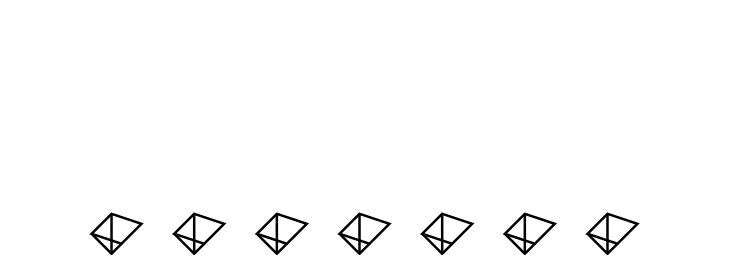
\includegraphics[width=\columnwidth]{images/atmo3d.pdf}
      \end{figure}
    \end{column}
  \end{columns}
\end{frame}

%%%%%%%%%%%%%%%%%%%%%%%%%%%%%%%%%%%%%%%%%%%%%%%%%%%%%%%

\subsection{Multi-Scattering Simulations}

\begin{frame}{Monte Carlo}
  \begin{figure}
    \centering
    \begin{overprint}
      \only<1>
      {\centerline{\def\svgwidth{0.5\linewidth}\small{\input{images/mc_method.pdf_tex}}}}
      \only<2>
      {\centerline{\includegraphics[height=7cm]{images/mc_result.pdf}}}
      \only<3>
      {\centerline{\def\svgwidth{0.5\linewidth}\small{\input{images/cross_section.pdf_tex}}}}
    \end{overprint}
  \end{figure}
\end{frame}

%%%%%%%%%%%%%%%%%%%%%%%%%%%%%%%%%%%%%%%%%%%%%%%%%%%%%%%

\subsection{Inverse Problem}

\begin{frame}{Inverse Problem}
  \begin{block}{Problem}
    Given a set of captured images, calculate the underlying aerosol
    distribution
  \end{block}
\end{frame}

%%%

\begin{frame}[label=objective]{Formulation}
  \begin{block}{Objective Function}
    \begin{equation*}
      \CostFunc{\DistUnknown}
      = \sum_{c=1}^{N_{\rm views}}
      \left\|
        \tikz[baseline]{ \node[na] (d1) {$\MaskSun$};}[{\bm i}^{\rm measured}_c - {\bm i}_c({\bm n})]
      \right\|^2_2  + \eta \tikz[baseline]{ \node[na] (d2) {$\Psi$};}({\bm n})
    \end{equation*}
  \end{block}
  \begin{block}{Estimated Aerosols}
    \begin{equation*}
      \DistEstimated =
      \argmin_{\DistUnknown \in \DistSet} \CostFunc{\DistUnknown}
    \end{equation*}
  \end{block}
  \begin{tikzpicture}[overlay] \pause
    \node[nodeblue] at (3,5.5) (s1) {\hyperlink{mask}{M.S. Mask}};
    \path[->] (s1) edge [bend left] (d1); \pause
    \node[nodeyellow] at (8,5.5)(s2) {\hyperlink{regularization}{Regularizer}};
    \path[->] (s2) edge [bend left] (d2);
  \end{tikzpicture}
\end{frame}

%%%

\begin{frame}{Challenge}
  \begin{figure}
    \centering
    \centerline{\includegraphics[height=7cm]{images/voxels3.pdf}}
  \end{figure}
\end{frame}

%%%

\begin{frame}[label=gradient]{Optimization}
  \begin{block}{Gradient}
    \begin{align*}
      \Grad{{\bm n}} E &= \\
      -&2\sum_{c=1}^{N_{\rm views}}
      \transpose{\left[{\bm J}_{{\bm i}_c}({\bm n})\right]} \transpose{\MaskSun}\MaskSun[{\bm i}^{\rm
        measured}_c - {\bm i}_c({\bm n})] + 2 \eta
      \transpose{\Laplacian}\transpose{{\bf W}}{\bf W}\Laplacian{\bm n}
    \end{align*}
  \end{block}
  \hfill\hyperlink{jacobian}{\beamergotobutton{Jacobian}}
\end{frame}

%%%

\begin{frame}{Parallelization}
  \begin{itemize}
  \item Processed using a computer cluster
  \item Each synthetic camera processed on a separate core
  \item Total 95 synthetic cameras
  \item A couple of hours to reconstruct 250K voxels
  \end{itemize}
\end{frame}

%%%

\begin{frame}{Results - Original Atmospheres}
  \centerline{\def\svgwidth{1.15\linewidth}\footnotesize{\input{images/atmo3d_original.pdf_tex}}}
  \centerline{\footnotesize Color represents aerosol density. The
    density units are $10^{6}~{\rm particles}/{\rm m}^3.$}
\end{frame}

%%%

\begin{frame}{Results - Single-scattering Simulations}
  \centerline{\def\svgwidth{1.15\linewidth}\footnotesize{\input{images/atmo3d_single.pdf_tex}}}
  \centerline{\footnotesize Color represents aerosol density. The
    density units are $10^{6}~{\rm particles}/{\rm m}^3.$}
\end{frame}

%%%

\begin{frame}{Results - Monte-Carlo Simulations}
  \centerline{\def\svgwidth{1.15\linewidth}\footnotesize{\input{images/atmo3d_mc.pdf_tex}}}
  \centerline{\footnotesize Color represents aerosol density. The
    density units are $10^{6}~{\rm particles}/{\rm m}^3.$}
\end{frame}

%%%%%%%%%%%%%%%%%%%%%%%%%%%%%%%%%%%%%%%%%%%%%%%%%%%%%%%%%%%%
%%%%%%%%%%%%%%%%%%%%%%%%%%%%%%%%%%%%%%%%%%%%%%%%%%%%%%%%%%%%

\section{Further Research Directions}

\subsection{Empirical Validation}

\begin{frame}[label=current]{Experiment}
  \begin{columns}[T]
    \begin{column}{.7\textwidth}
      \begin{itemize}
      \item Grab multiple images from moving car
      \item Images registered using GPS and/or SfM tools
      \item Compare to ground truth
        \begin{itemize}
        \item MISR
        \item LIDAR
        \item AERONET
        \end{itemize}
      \end{itemize}
    \end{column}
    \begin{column}{.3\textwidth}
      \centering
      \includegraphics[height=0.30\textheight]{DSC_0688.JPG}
      \captionof{figure}{}
      \includegraphics[height=0.30\textheight]{AERONET.jpg}
      \captionof{figure}{}
    \end{column}
  \end{columns}
\end{frame}

%%%%%%%%%%%%%%%%%%%%%%%%%%%%%%%%%%%%%%%%%%%%%%%%%%%%%%%

\subsection{Inverse Problem}

\begin{frame}{Model Extension}
  \begin{itemize}
  \item Multiple particles
    \begin{itemize}
    \item Martonchik at el. 1998
    \end{itemize}
  \item Improve algorithm speed
  \item Account for Multiple-Scattering
  \item Cloudy Skies
  \end{itemize}

\end{frame}

%%%%%%%%%%%%%%%%%%%%%%%%%%%%%%%%%%%%%%%%%%%%%%%%%%%%%%%

\subsection{Aerosols in Partly Cloudy Skies}

\begin{frame}{Clouds}
  \begin{columns}[T]
    \begin{column}{.6\textwidth}
      \begin{itemize}
      \item High Optical Depth
        \begin{itemize}
        \item Single-Scattering approximation not-valid.
        \end{itemize}
      \item Affect radiation transfer:
        \begin{itemize}
        \item Cast shadows
        \item Reflect light
        \end{itemize}
      \end{itemize}
    \end{column}
    \begin{column}{.4\textwidth}
      \includegraphics[height=0.40\textheight]{clouds.jpg}
    \end{column}
  \end{columns}
\end{frame}

%%%

\begin{frame}{Reconstruction}

  \begin{itemize}
  \item Separate reconstruction
    \begin{itemize}
    \item SfM - Structure from Motion 
    \item Visual Hull
    \end{itemize}

  \item Model extension
    \begin{itemize}
    \item Calculate effective phase function
    \item Add as a separate source
    \end{itemize}
  \end{itemize}

\end{frame}

%%%

\begin{frame}[label=current]{Reconstructed Clouds}
  \centerline{\movie[height=7cm, width=12cm, poster, autostart]{Cloud Reconstruction}{clouds.avi}}
\end{frame}

%%%

\begin{frame}{Thank You}
  \begin{center}
    Thank You!
  \end{center}
\end{frame}

%%%%%%%%%%%%%%%%%%%%%%%%%%%%%%%%%%%%%%%%%%%%%%%%%%%%%%%%%%%%
%%%%%%%%%%%%%%%%%%%%%% appendix %%%%%%%%%%%%%%%%%%%%%%%%%%%%
%%%%%%%%%%%%%%%%%%%%%%%%%%%%%%%%%%%%%%%%%%%%%%%%%%%%%%%%%%%%

\appendix

\begin{frame}[label=jacobian]{Jacobian (Differentiation)}
  \begin{block}{Jacobian Equation}
    \begin{align*}
      {\bm J}_{{\bm i}_c}({\bm n}) &= \\
      &L^{\rm TOA}{\sigma}^{\rm
        aerosol}({\bf A}-{\bf B}) \OpDiag{\exp[-(\vect{\tau}_c^{\rm air} +
        {\sigma}^{\rm aerosol} {\bm D}_c {\bm n})]}
      \transpose{{\vect{\Pi}}_c}
    \end{align*}
    where
    \begin{align*}
      {\bf A} &= \varpi^{\rm aerosol}
      \OpDiag{ P_g^{\rm aerosol}(\vect{\Phi}^{\rm scatter}_c)} \\
      {\bf B} &= \transpose{{\bm D}_c}
      \OpDiag{[\tilde{\vect{\alpha}}^{\rm air}_c + \varpi^{\rm
          aerosol}\sigma^{\rm aerosol} P^{\rm aerosol}_g(\vect{\Phi}^{\rm
          scatter}_c) \odot{\bm n}    ]}
    \end{align*}
  \end{block}
  \hfill\hyperlink{gradient}{\beamerreturnbutton{Return}}
\end{frame}

\begin{frame}[label=mask]{Multi-Scattering Mask}
  \begin{itemize}
  \item Weight error by Single-Scattering dominance
  \item Calculated empirically
  \end{itemize}
  \centerline{\includegraphics[height=4cm]{images/sun_mask.pdf}}
  \hfill\hyperlink{objective<3>}{\beamerreturnbutton{Return}} 
\end{frame}

\begin{frame}[label=regularization]{Regularization}
  \begin{itemize}
  \item Aerosol distributions are usually fuzzy
  \item 3D Laplacian enforces {\em smoothness}: $\Laplacian{\bm n} = \| \nabla^2{\bm  n}\|^2_2$
  \item Weighted by altitude: $w(k)=\exp\left[-h(k)/H^\mathrm{smooth}\right]$
  \item Regularization by $\Psi({\bm n}) = \| {\bf W} \Laplacian{\bm n}\|^2_2$
  \end{itemize}

  \hfill\hyperlink{objective<3>}{\beamerreturnbutton{Return}}
\end{frame}

%%%%%%%%%%%%%%%%%%%%%%%%%%%%%%%%%%%%%%%%%%%%%%%%%%%%%%%%%%%%
%%%%%%%%%%%%%%%%%%%%%%%% end %%%%%%%%%%%%%%%%%%%%%%%%%%%%%%%
%%%%%%%%%%%%%%%%%%%%%%%%%%%%%%%%%%%%%%%%%%%%%%%%%%%%%%%%%%%%

\end{document}

